% @Author: AnthonyKenny98
% @Date:   2020-03-01 18:51:24
% @Last Modified by:   AnthonyKenny98
% @Last Modified time: 2020-04-11 01:27:28
\subsection{RISC-V}

    \gls{RISC-V} (pronounced ``risk-five'') was developed at the University of California, Berkeley. It is established on the principles of RISC as an open-source and extendable \gls{ISA} for research and education. It was designed with application specific processors in mind, as they developed a highly flexible and extendable base \gls{ISA} around which research and acceleration efforts could be based.

    The motiviation behind designing RISC-V was largely due to the following disadvantages of commercially popular \glspl{ISA}.\cite{Isa2012}.
    \begin{itemize}
    \item \textbf{Commercial ISAs are proprietary.} Owners of commercial ISAs carefully guard their intellectual property and will not share implementations. 
    \item \textbf{Commercial ISAs come and go.} Many once-popular commercial ISAs have since fallen out of fashion or are not even in production any more. Lingering intellectual property issues interefere with the ability of third-parties to continue supporting the ISA. While an open source \gls{ISA} may also lose popularity, interested parties can continue to use and support the ISA without interference.
    \item \textbf{Popular commercial ISAs were not designed for extendibility.} There exist almost no ISAs that support extendibility for general purpose computing systems, allowing for no application specific optimizations at the instruction set level.
    \end{itemize}

    % RISC-V is designed cleverly in a modular way, with a set of base instruction sets and a set of standard extensions. As a result, processors can be designed to only implement the instruction groups it requires, saving time, space and power on instructions that won't be used. In addition, another goal of RISC-V is to provide a basis for more specialized instruction-set extensions or more customized accelerators. This is described in the most recent \textit{RISC-V Instruction Set Manual} \cite{Waterman2019}. This is a powerful feature, as it does not break any software compatability, but allows for designers to easily follow the steps outlined in Figure \ref{fig:extendingRISCV}. From a \gls{hardware acceleration} point of view, this is particularly useful as it allows the designer to directly invoke whatever functional unit or accelerator they implement from assembly code.
    
    % % @Author: AnthonyKenny98
% @Date:   2020-03-01 10:28:34
% @Last Modified by:   AnthonyKenny98
% @Last Modified time: 2020-03-01 10:32:45
\begin{figure}[H]
\begin{center}
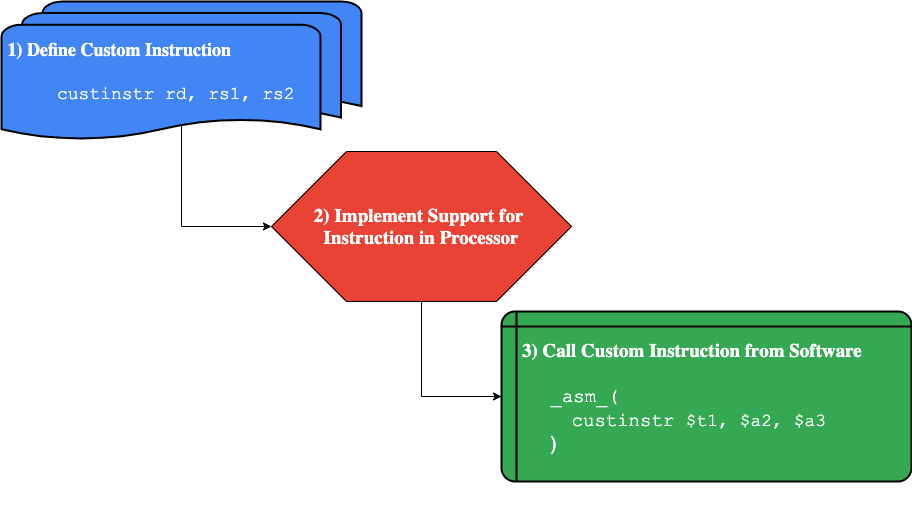
\includegraphics[width=0.9\linewidth]{chapters/chapter1/img/extendingRISCV.png}
\caption{Typical Process of Adding Non-Standard Extension to RISC-V ISA}
\label{fig:extendingRISCV}
\end{center}
\end{figure}

    The overall design of RISC-V can be broken down into 3 characteristics that address the aforementioned limitations of commercial \glspl{ISA}: Open-source, extendibility, and modularity.

    \subsubsection{Open-Source}
        Open-source refers to software that the owner of which has granted permission for anybody to study, alter, or distribute the software for any purpose. Often, this means projects are developed in a collaborative public manner. What this means for an ISA is that RISC-V implementations are often publicly available and improved upon by developers for their own purposes. Building a high-performance processor from scratch is an arduous, expensive project. Open-source implementations allow developers to build upon existing implementations without the legwork of implementing a processor from scratch.

    \subsubsection{Extendability}
        RISC-V is designed to be extendable. This means that developers can add their own instructions to the Instruction Set and implement those new instructions in a processor. This processor should still be able to run all other RISC-V compiled programs, along with a set of programs for which it is specifically optimized. This backwards compatibility means that an extended ISA is not just a new ISA. 

    \subsubsection{Modularity}
        Finally, RISC-V was designed to be relatively easy to implement. It is broken down into small ``base'' \glspl{ISA} which can then have any number of standard and non-standard extensions added to them. These base ISAs are not designed in such a way to overarchitect for a certain type of microarchitecure. \textbf{Standard extensions} are those that are generally useful and that are designed to not conflict with any other standard extensions. \textbf{Non-standard extensions} are those that may be highly specialized and may conflict with other standard or non-standard extensions. One way to think about it is that standard extensions would improve any computer and are endorsed by the RISC-V organization, whereas non-standard extensions are developed for very specific purposes, such as motion planning acceleration. This modularity and flexibility is part of what makes RISC-V such an attractive proposition for specialized computer architecture. Figure \ref{fig:modules} demonstrates this modularity.

        % @Author: AnthonyKenny98
% @Date:   2020-04-09 12:52:23
% @Last Modified by:   AnthonyKenny98
% @Last Modified time: 2020-04-09 20:19:52
\begin{figure}[H]
\begin{centering}
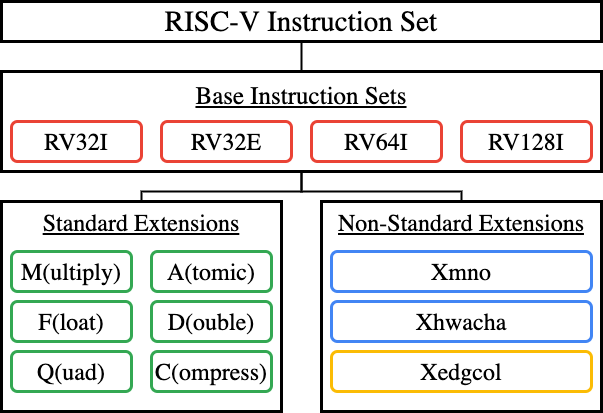
\includegraphics[width=0.8\linewidth]{chapters/chapter4/img/modules.png}
\mycaption{RISC-V ISA Modularity}{. It is clear that the RISC-V ISA is in fact a family of ISAs. Each is based on one of the ``base'' ISAs, which are each the smallest possible ISA to run just about any program. For more instructions and thus, better performance, any number of Standard or Non-Standard Extensions can be implemented on top of a base ISA.}
\label{fig:modules}
\end{centering}
\end{figure}

\subsection{RV32I}
    The RV32I (Short for RISC-V 32-Bit Integer) base \gls{ISA} is a small \gls{ISA} of only 40 unique instructions, but sufficient to support modern operating systems. It has 32 registers, \texttt{x0-x32}, each 32-bits wide. \texttt{x0} is a hard-wired 0, and there is also another register dedicated for the program count. 


    The following is an excerpt from the RISC-V Specification, outlining the RV32I base integer instruction set \cite{Waterman2019}:
    \begin{quote}{}
        \small{RV32I was designed to be sufficient to form a compiler target and to support modern operating system environments. The ISA was also designed to reduce the hardware required in a minimal implementation. RV32I contains 40 unique instructions, though a simple implementation might \dots [reduce] base instruction count to 38 total. RV32I can emulate almost any other ISA extension \dots \\
        Subsets of the base integer ISA might be useful for pedagogical purposes, but the base has been defined such that there should be little incentive to subset a real hardware implementation \dots}
    \end{quote}

    RV32I was chosen as the base ISA for this project. The edge collision custom extension would be defined primarily extend the RV32I base ISA. Figure \ref{fig:systemOverviewUpdated} is an updated system diagram of the overall project.

    % @Author: AnthonyKenny98
% @Date:   2020-04-10 18:50:27
% @Last Modified by:   AnthonyKenny98
% @Last Modified time: 2020-04-10 18:52:47
\begin{figure}[H]
\begin{center}
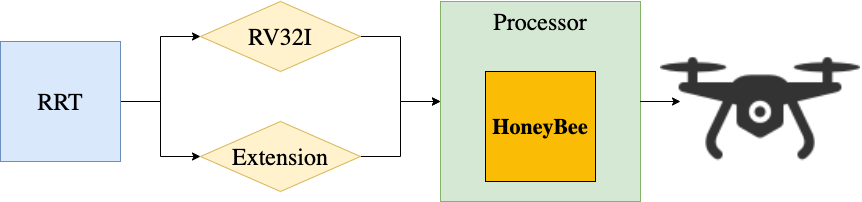
\includegraphics[width=0.9\linewidth]{chapters/chapter4/img/systemOverviewUpdated.png}
\mycaption{Updated System Overview}{ showing how RRT is compiled through the RV32I ISA with the edge collision extension.}
\label{fig:systemOverviewUpdated}
\end{center}
\end{figure}

    % \subsubsection*{Registers}
    %     RV32I defines 32 unprivileged registers, each 32 bits wide. They are designated \texttt{x0-x31}, where \texttt{x0} is a hard-wired value of $0$, and registers \texttt{x1-x31} hold values that various instructions use. RISC-V uses the load-store method, meaning that all operations perform on two registers or a register and an immediate, rather than performing operations directly on memory addresses. In addition, a 33rd unprivileged register is a program counter \texttt{pc}. 
        % Table \ref{table:rv32i_reg} shows the register state for the RV32I Base Integer Instruction Set.
        % % @Author: AnthonyKenny98
% @Date:   2020-03-01 18:36:35
% @Last Modified by:   AnthonyKenny98
% @Last Modified time: 2020-03-01 19:33:20
\begin{table}[H]
\begin{center}
\begin{tabular}{|p{.15\linewidth}|p{.15\linewidth}|p{.4\linewidth}|}
    \hline
    \textbf{Register}   & \textbf{ABI Name}  & \textbf{Description} \\
    \hline
    \texttt{x0}  & \texttt{zero} & Hard-wired zero \\
    \texttt{x1}& \texttt{ra}& Return address\\
    \texttt{x2}& \texttt{sp} & Stack pointer\\
    \texttt{x3}& \texttt{gp}&Global pointer\\
    \texttt{x4}& \texttt{tp}& Thread pointer\\
    \texttt{x5-7}& \texttt{t0-2}&Temporaries\\
    \texttt{x8}& \texttt{s0/fp}&Saved register/Frame pointer\\
    \texttt{x9}&\texttt{s1} &Saved register\\
    \texttt{x10-11}&\texttt{a0-1}&Function arguments/return values\\
    \texttt{x12-17}&\texttt{a2-7}&Function arguments\\
    \texttt{x18-27}&\texttt{s2-11}&Saved registers\\
    \texttt{x28-31}&\texttt{t3-6}&Temporaries\\
    \hline
    \texttt{pc} & \texttt{pc} & Program counter \\
    \hline
\end{tabular}
\caption{Register State for RV32I Base Instruction Set}
\label{table:rv32i_reg}
\end{center}
\end{table}

    % \subsubsection{Instructions}
    %     RV32I defines 40 instructions that together are sufficient to run most modern operating systems.
    %     Table \ref{table:rv32i_instr_format} demonstrates the format of each different instruction type. 
    %     % @Author: AnthonyKenny98
% @Date:   2020-03-01 19:13:03
% @Last Modified by:   AnthonyKenny98
% @Last Modified time: 2020-03-01 19:32:00
\begin{table}[H]
\begin{center}
    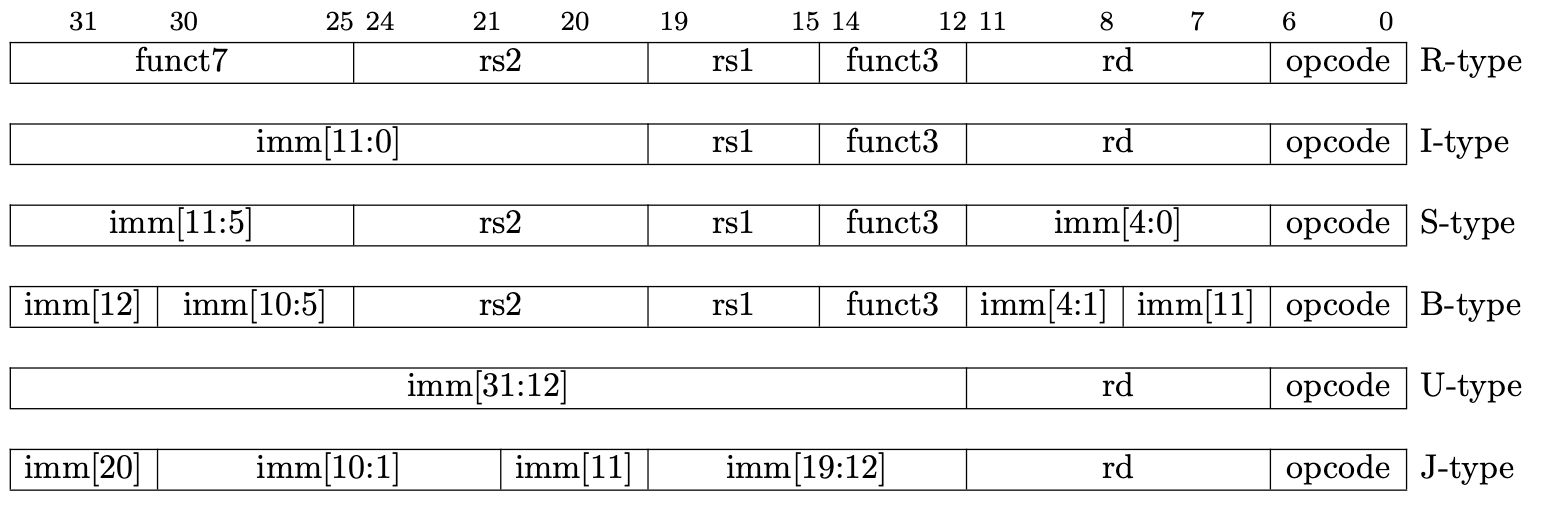
\includegraphics[draft=false,width=\linewidth]{chapters/chapter4/img/rv32i_instr_format.png}
    \caption{RV32I Base Instruction Formats}
    \label{table:rv32i_instr_format}
\end{center}
\end{table}


